\section{Expansion Model}

In the expansive behavior of DEF and ASR, the expanse is caused by strains generated from within the concrete when there is no external loading.

One of the similar behavior in previous research is the strength development due to autogenous shrinkage in high strength concrete, which was carried out by Osakabe et al., (2014)\cite{Osakabe}. The concept of initial strain in RBSM has been successfully utilized in the simulation of the behavior of autogenous shrinkage in high strength concrete.

The same concept of initial strain is utilized in the present of ASR and DEF expanse behavior carried out by L.EDDY et al. in 2016\cite{Eddy}. Characteristic map cracking pattern in ASR simulation was presented successfully, while the DEF simulation results do not match well with the typical map cracking pattern observed in the real concrete.

The concept of the initial strain used in this simulation is based on the case where a specimen expansion occurs without any constraint.

According to 3D RBSM developed by Nagai et al. (2005)\cite{Nagai}, the first step is the calculation of actual force, which supposed to be calculated by solving strain, stress and force matrices of all elements in sequence based on input data and boundary condition.

Iteration is then performend until this force under the acceptable limit with an external force. When the convergence condition is reached, the same sequence will be performed for the next step.

In our simulation, one additional step of introducing the initial strain is added here to simulate the behavior of expansion. Then, Stresses due to this initial strain are calculated in the next step, with considering the initial strain added. After the stress is calculated, the initial strain added up earlier will be subtracted, before the forces are calculated.

The illustration of introducing initial strain is shown in the Figure \ref{fig:Flow}.

\begin{figure}[ht!]
    \centering
    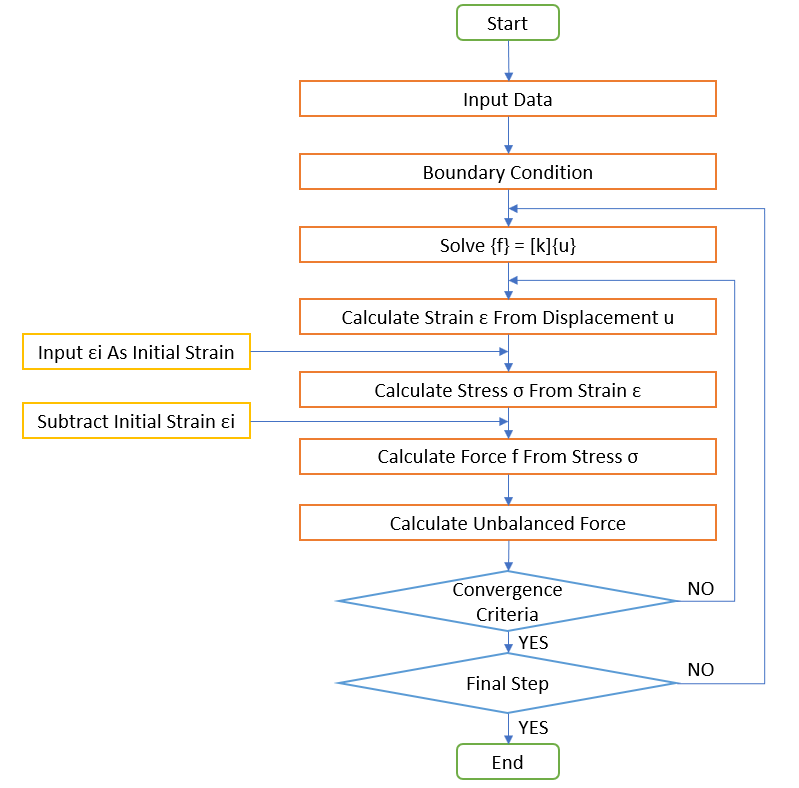
\includegraphics[width=1.0\linewidth]{Files/Method/flow.png}
    \caption{Flow Diagram of Simulation of Expansion Through RBSM}
    \label{fig:Flow}
\end{figure}


For ASR and DEF, the initial strains are introduced at different interfaces in concrete.

Expansion is giving to simulative the behavior of model up to 1.3\% expansion(in one dimensional).

To calculate the one dimensional expansion, here 2 elements located at center of left and right surface, seperately, are selected, their distant before and after expansion is recorded.

\begin{figure}[h!]
\centering
%*******
\begin{subfigure}{.4\textwidth}
  \centering
  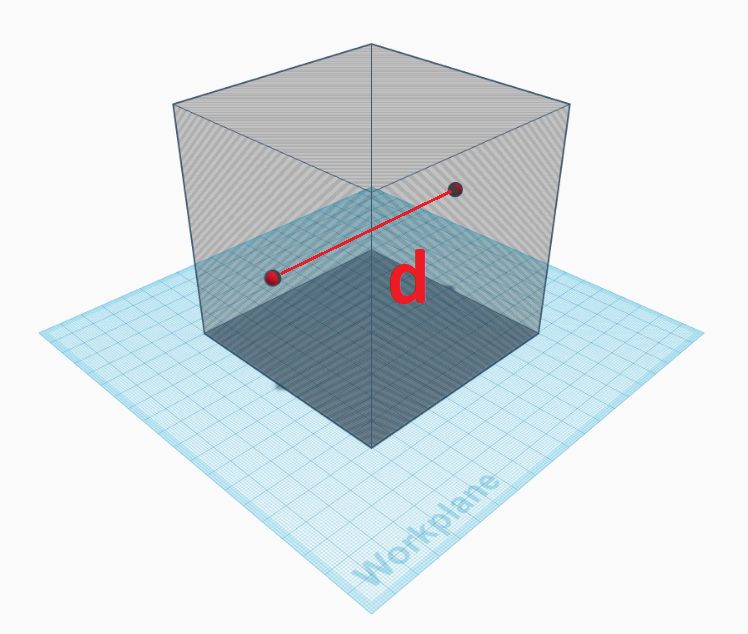
\includegraphics[width=1.0\linewidth]{Files/Method/dis0.png}
\caption{3D View}
\end{subfigure}%
%*******
\begin{subfigure}{.4\textwidth}
  \centering
  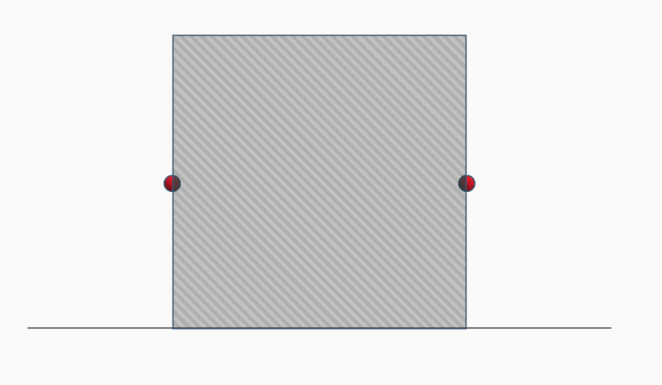
\includegraphics[width=1.0\linewidth]{Files/Method/dis1.png}
\caption{Cross Section View}
\end{subfigure}%
%*******
\caption{Points Selected For Calculation One-dimensional Expansion}
\end{figure}

\subsection{ASR Expansion Behavior In Simulation}

For ASR expansion, the expanse is generated at the location of interfaces between mortar and aggregate. The concept of the initial strain is used here to introduce the expansion.

As we consider the ratio of reactive aggregate may differ the behavior of the model in ASR expansion,  cases of different percentage aggregate expanse are simulated and cross-compared. The reactive aggregates are also chosen randomly.

\begin{figure}
  \centering
  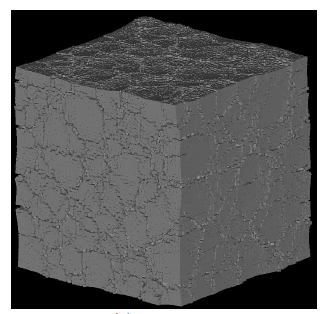
\includegraphics[width=0.4\linewidth]{Files/Background/EDDY_ASR.png}
  \caption{Characteristic Map Cracking Pattern of ASR bu RBSM Simulation, L.EDDY et al. (2016)}
\end{figure}

As in the research done by L.EDDY et al. (2016)\cite{Eddy}, the desired characteristic map cracking pattern of ASR expansion has already achieved in this method. In this simulation, the discussion is focused on the relationship between cracking pattern with aggregate percentage, reactive aggregate, expanding ratio, also the residual mechanical properties of ASR-damaged concrete.

\subsection{DEF Expansion Behavior In Simulation}

Similar model and mechanism are also applied in the simulation of DEF  type expansion. Following the popular theory of expansion in DEF  is caused by expansion of paste, initial strain here is given to the interfaces between mortar elements to present the DEF expansion.

According to the previous study done by L.EDDY et al, simple uniformed paste expansion theory need improvement. Whether for cases giving initial strain to 100\%, 50\% or 25\% random faces of mortar chosen to expanse, the surface of expanded concrete does not match with the actual cracking pattern.

It is well established that high early temperature experienced by the concrete is the most important factor inducing DEF in concrete. (Ghorab et al .,1980\cite{Ghorab}, Heinz, D et al., 1986\ref{Heinz} etc.)

The research done by Anupam (2016)\cite{Awasthi} confirmed the rising of the temperature inside concrete due to combination effect of steam curing and heat of hydration inside the concrete is not uniform. Both the simulation result is done by Astea Macs (FEM based non-linear thermal stress analysis program developed by Research Center of Computational Mechanics, Japan) and the field measurement of temperature rising process inside concrete during steam curing in a concrete plant located in India shows the un-uniformed distribution of maximum temperature experienced. The temperature in the center of the concrete structure is significantly higher than the outer part.

\begin{figure}[ht!]
\centering
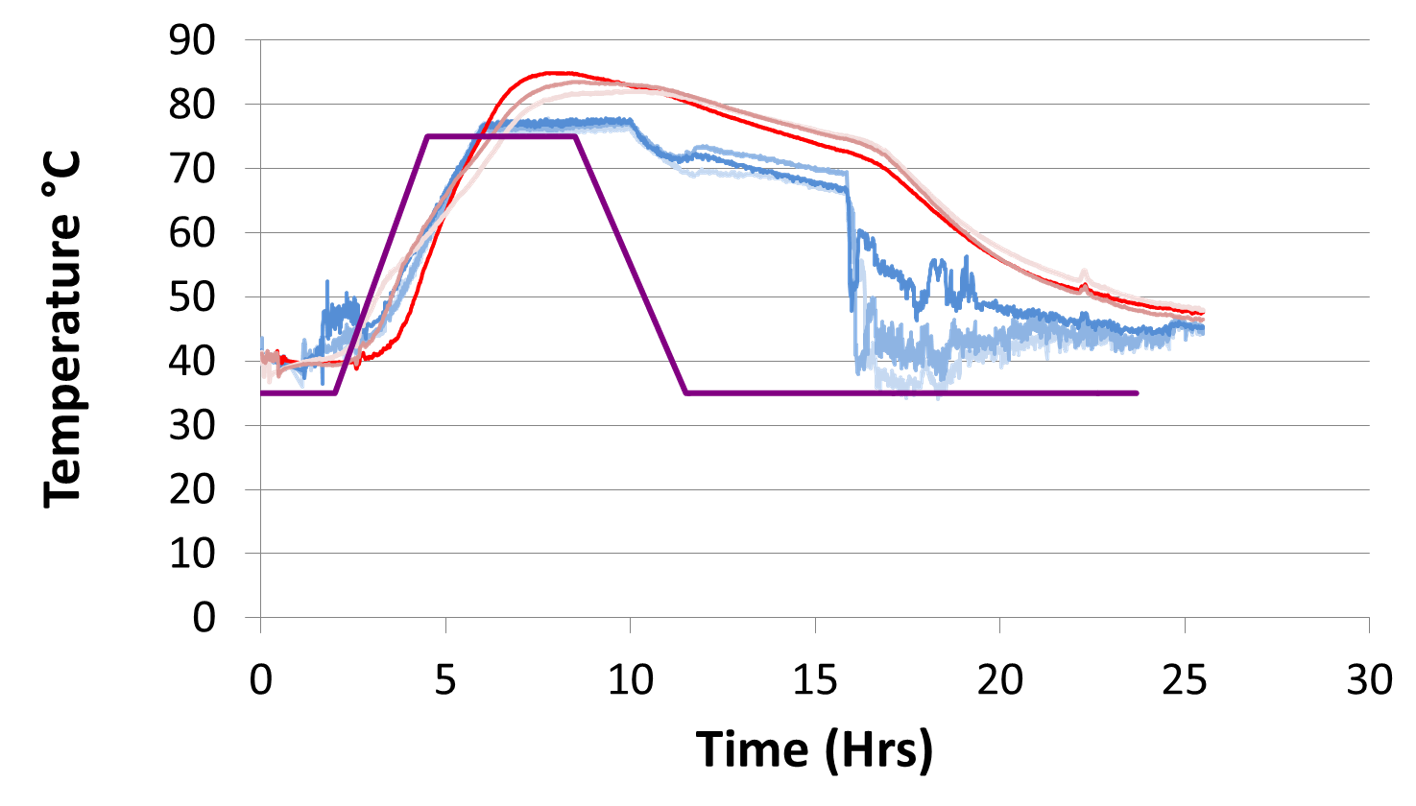
\includegraphics[width=.6\linewidth]{Files/Background/Anupam_2.png}
  \caption{Result of Temperature Measurement, A.AWASTHI 2016}
  \label{fig:temp_measurement}
\end{figure}


The cracking pattern in DEF damaged concrete, recorded by Anupam (2016)\cite{Awasthi}, also suggested the possibility of non-uniformed expansion happens in DEF damaged concrete structure. The cracking concentrated in the outer part of the structure, while the inner part remained undamaged, showing the trend of larger expansion happening in the inner part of the concrete paste.

\begin{figure}[ht!]
\centering
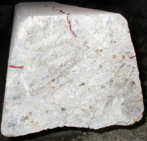
\includegraphics[width=.4\linewidth]{Files/Background/Anupam_5.png}
  \caption{Section View of DEF Damaged Concrete Sleeper, A.AWASTHI 2016}
  \label{fig:section_view}
\end{figure}

Considering the effect of temperature on triggering  DEF expansion and its characteristic cracking pattern, for DEF simulation, uniform expansion does not quite fit with the real situation. The expansion inside concrete structure supposes to be much severe than the outer part. For which here in this research non-uniformed expanding is introduced by giving a different amount of DEF initial strain considering the location of element.


The inner part of the model will be giving larger initial strain,  present the higher maximum temperature experienced, while the outer part mortar will be giving small or none initial strain.

\begin{figure}[ht]
\centering
    %*******
    \begin{subfigure}{.33\textwidth}
      \centering
      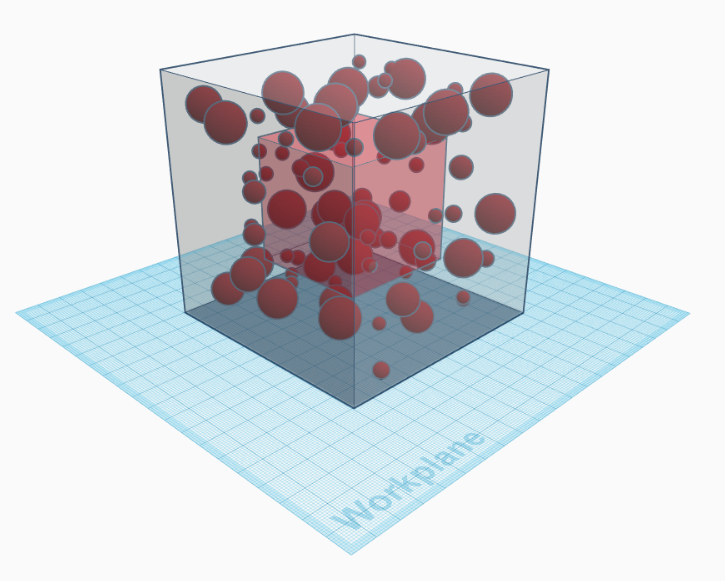
\includegraphics[width=.8\linewidth]{Files/DEF_X/X0_3d.png}
    \end{subfigure}%
    %*******
    \begin{subfigure}{.33\textwidth}
      \centering
      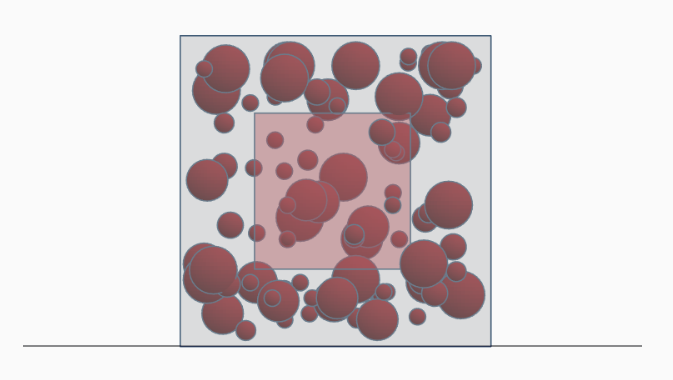
\includegraphics[width=.8\linewidth]{Files/DEF_X/X0_3ds.png}
    \end{subfigure}
    %*******
  \caption{50x50x50mm DEF intensified part range}
  \label{fig:non-uniform DEF}
  \end{figure}


%*******10********20********30********40********50********60********70********80
